\documentclass[10pt]{standalone}
\usepackage{amsmath,amsfonts,amssymb} % For math equations, theorems, symbols, etc

\usepackage{makecell} % allows line breaking in table cells
\usepackage{pifont}
\usepackage{float}
\usepackage{nameref}
\usepackage[nice]{nicefrac}
\usepackage{marginnote}
\usepackage{stackengine} % needed for \belowbaseline, which is used when aligning matrices by their top row
\usepackage[breakwords]{truncate}
\usepackage{etoolbox} % Needed to make marginnotes always appear in left margin
\newcommand*{\diff}{\mathop{}\:\!d}

\usepackage{graphicx} % Required for including pictures
\usepackage{colortbl}
\arrayrulecolor{gray} % Make block matrices have gray rules

\graphicspath{{images/}} % Specifies the directory where pictures are stored

\usepackage{tikz} % Required for drawing custom shapes
\usepackage{tikz-3dplot} %requires 3dplot.sty to be in same directory, or in your LaTeX installation
\usetikzlibrary{arrows.meta}
\usetikzlibrary{shapes}
\usetikzlibrary{calc,fadings,decorations.pathreplacing,angles,positioning,fit,backgrounds,fpu}
\usepackage{pgfplots}
\pgfplotsset{compat=1.12}
\usepgfplotslibrary{fillbetween}

\newcommand{\RightAngle}[5][3pt]{%
	\draw[#5] ($#3!#1!#2$)
	--($ #3!2!($($#3!#1!#2$)!.5!($#3!#1!#4$)$) $)
	--($#3!#1!#4$) ;
}

\newcommand{\transformarrow}[1]{$\xrightarrow{\ \ \text{#1} \ }$}

% Polynomial long division
\newcommand\Mydiv[2]{%
	\strut#1\kern.25em\smash{\raise.3ex\hbox{\big)}}\mkern-8mu
	\overline{\enspace\strut#2}}

% For drawing graphs in tikz
\tikzstyle{ocrenode}=[draw=ocre,circle,fill=locre,path fading=fade right,text=black,minimum width=10pt]
\tikzstyle{grennode}=[draw=gren,circle,fill=lgren,path fading=fade right,text=black,minimum width=10pt]
\tikzstyle{purpnode}=[draw=purp,circle,fill=lpurp,path fading=fade right,text=black,minimum width=10pt]
\tikzstyle{ocrenoderect}=[draw=ocre,rectangle,rounded corners=5pt,inner sep=6pt,fill=locre,path fading=fade right,text=black,minimum width=10pt]
\tikzstyle{grennoderect}=[draw=gren,rectangle,rounded corners=5pt,inner sep=6pt,fill=lgren,path fading=fade right,text=black,minimum width=10pt]
\tikzstyle{purpnoderect}=[draw=purp,rectangle,rounded corners=5pt,inner sep=6pt,fill=lpurp,path fading=fade right,text=black,minimum width=10pt]
\definecolor{darkorangeback}{RGB}{128,54,0}

\usepackage[english]{babel} % English language/hyphenation
\usepackage{gensymb} % gives the degree symbol

\usepackage{enumitem} % Customize lists
\setlist{nolistsep} % Reduce spacing between bullet points and numbered lists
\usepackage[outline]{contour}

\usepackage{booktabs} % Required for nicer horizontal rules in tables

%% The next command allows for vertical centering of images next to each other in figures.
\newcommand*{\vcenteredhbox}[1]{\begingroup
	\setbox0=\hbox{#1}\parbox{\wd0}{\box0}\endgroup}

\usepackage{multirow} % Used for some subfigure environments when one image is huge
\usepackage{multicol} % Used for enumerate in exercises with multiple images to put them side by side
\usepackage{systeme}\sysdelim.. % Used for typesetting systems of linear equations

\usepackage{xcolor} % Required for specifying colors by name
\usepackage{colortbl}
\definecolor{ocre}{RGB}{0,96,128} % Define the blue color used for highlighting throughout the book
\colorlet{chapcolor}{ocre}
\definecolor{orng}{RGB}{224,112,0} % Define the orange color used for highlighting throughout the book
\definecolor{gren}{RGB}{0,128,0} % Define the green color used for highlighting throughout the book
\definecolor{purp}{RGB}{112,0,112} % Define the purple color used for highlighting throughout the book
\definecolor{dred}{RGB}{164,28,0} % Define the red color used for highlighting throughout the book
\definecolor{locre}{RGB}{128,176,192} % Light blue
\definecolor{lorng}{RGB}{236,184,128} % Light orange
\definecolor{lgren}{RGB}{128,192,128} % Light green
\definecolor{lpurp}{RGB}{184,128,184} % Light purple
\definecolor{lgray}{RGB}{192,192,192} % Light gray
\definecolor{llgray}{RGB}{242,242,242} % Really light (background) gray
\interfootnotelinepenalty=10000 % prevent long footnotes from being split across two pages


% Commands for making letter grids in proofs
\newcommand{\letternode}[3]{\node[anchor=center] at (#1,#2){\fontsize{18}{18}\sffamily\bfseries\contour{black}{\textcolor{ocre!40}{#3}}};}
\newcommand{\colorletternode}[4]{\node[anchor=center] at (#2,#3){\fontsize{18}{18}\sffamily\bfseries\contour{black}{\textcolor{#1!40}{#4}}};}
\newcommand{\sizecolorletternode}[5]{\node[anchor=center] at (#2,#3){\fontsize{#5}{#5}\sffamily\bfseries\contour{black}{\textcolor{#1!40}{#4}}};} 
\newcommand{\gridbox}[2]{\setlength{\fboxsep}{0mm}
	\setlength{\fboxrule}{#1}\fcolorbox{gridgray}{gridgray}{#2}}



% Lets you draw an arc of an ellipse
% From https://tex.stackexchange.com/questions/123158/tikz-using-the-ellipse-command-with-a-start-and-end-angle-instead-of-an-arc
\tikzset{
	partial ellipse/.style args={#1:#2:#3}{
		insert path={+ (#1:#3) arc (#1:#2:#3)}
	}
}


\newcommand{\gliderarrow}[1]{\color{black}{$\xrightarrow{\text{
\includegraphics[width=0.25cm]{../glider.png} #1}}$}}



% DEFINES A GLIDER SHAPE FOR USE IN TIKZ
\def\glider#1#2#3{
	\begin{scope}[shift={#1}, rotate=#2, scale=#3]
		\fill[black](0,0) -- (1,0) -- (1,1) -- (0,1) -- cycle;
		\fill[black](8/7+0,0) -- (8/7+1,0) -- (8/7+1,1) -- (8/7+0,1) -- cycle;
		\fill[black](16/7+0,0) -- (16/7+1,0) -- (16/7+1,1) -- (16/7+0,1) -- cycle;
		\fill[black](16/7+0,8/7+0) -- (16/7+1,8/7+0) -- (16/7+1,8/7+1) -- (16/7+0,8/7+1) -- cycle;
		\fill[black](8/7+0,16/7+0) -- (8/7+1,16/7+0) -- (8/7+1,16/7+1) -- (8/7+0,16/7+1) -- cycle;
\end{scope}}
\def\lwss#1#2#3{
	\begin{scope}[shift={#1}, rotate=#2, scale=#3]
		\fill[black](0,0) -- (1,0) -- (1,1) -- (0,1) -- cycle;
		\fill[black](8/7+0,0) -- (8/7+1,0) -- (8/7+1,1) -- (8/7+0,1) -- cycle;
		\fill[black](16/7+0,0) -- (16/7+1,0) -- (16/7+1,1) -- (16/7+0,1) -- cycle;
		\fill[black](24/7+0,0) -- (24/7+1,0) -- (24/7+1,1) -- (24/7+0,1) -- cycle;
		\fill[black](32/7+0,8/7+0) -- (32/7+1,8/7+0) -- (32/7+1,8/7+1) -- (32/7+0,8/7+1) -- cycle;
		\fill[black](0,8/7+0) -- (1,8/7+0) -- (1,8/7+1) -- (0,8/7+1) -- cycle;
		\fill[black](0,16/7+0) -- (1,16/7+0) -- (1,16/7+1) -- (0,16/7+1) -- cycle;
		\fill[black](8/7+0,24/7+0) -- (8/7+1,24/7+0) -- (8/7+1,24/7+1) -- (8/7+0,24/7+1) -- cycle;
		\fill[black](32/7+0,24/7+0) -- (32/7+1,24/7+0) -- (32/7+1,24/7+1) -- (32/7+0,24/7+1) -- cycle;
\end{scope}}
\def\mwss#1#2#3{
	\begin{scope}[shift={#1}, rotate=#2, scale=#3]
		\fill[black](0,0) -- (1,0) -- (1,1) -- (0,1) -- cycle;
		\fill[black](8/7+0,0) -- (8/7+1,0) -- (8/7+1,1) -- (8/7+0,1) -- cycle;
		\fill[black](16/7+0,0) -- (16/7+1,0) -- (16/7+1,1) -- (16/7+0,1) -- cycle;
		\fill[black](24/7+0,0) -- (24/7+1,0) -- (24/7+1,1) -- (24/7+0,1) -- cycle;
		\fill[black](32/7+0,0) -- (32/7+1,0) -- (32/7+1,1) -- (32/7+0,1) -- cycle;
		\fill[black](40/7+0,8/7+0) -- (40/7+1,8/7+0) -- (40/7+1,8/7+1) -- (40/7+0,8/7+1) -- cycle;
		\fill[black](0,8/7+0) -- (1,8/7+0) -- (1,8/7+1) -- (0,8/7+1) -- cycle;
		\fill[black](0,16/7+0) -- (1,16/7+0) -- (1,16/7+1) -- (0,16/7+1) -- cycle;
		\fill[black](8/7+0,24/7+0) -- (8/7+1,24/7+0) -- (8/7+1,24/7+1) -- (8/7+0,24/7+1) -- cycle;
		\fill[black](24/7+0,32/7+0) -- (24/7+1,32/7+0) -- (24/7+1,32/7+1) -- (24/7+0,32/7+1) -- cycle;
		\fill[black](40/7+0,24/7+0) -- (40/7+1,24/7+0) -- (40/7+1,24/7+1) -- (40/7+0,24/7+1) -- cycle;
\end{scope}}
% DEFINES A BLOCK SHAPE FOR USE IN TIKZ
\def\golblock#1#2#3{
\begin{scope}[shift={#1}, scale=#3]
\fill[#2](0,0) -- (1,0) -- (1,1) -- (0,1) -- cycle;
\fill[#2](8/7+0,0) -- (8/7+1,0) -- (8/7+1,1) -- (8/7+0,1) -- cycle;
\fill[#2](0,8/7+0) -- (1,8/7+0) -- (1,8/7+1) -- (0,8/7+1) -- cycle;
\fill[#2](8/7+0,8/7+0) -- (8/7+1,8/7+0) -- (8/7+1,8/7+1) -- (8/7+0,8/7+1) -- cycle;
\end{scope}}


%----------------------------------------------------------------------------------------
%	FONTS
%----------------------------------------------------------------------------------------

\newcommand{\phantomsectiontotoc}[1]{%
	\addcontentsline{toc}{section}{\protect\numberline{\thesection}{#1}}%
}

% Three colors used in tables
\definecolor{gridgray}{RGB}{192,192,192}
\definecolor{medgray}{RGB}{128,128,128}
\definecolor{redback}{RGB}{255,168,168}
\definecolor{redback2}{RGB}{128,0,0}
\definecolor{greenback}{RGB}{168,255,168}
\definecolor{greenpastel}{RGB}{210,255,210}
\definecolor{greenback2}{RGB}{0,192,0}
\definecolor{darkgreenback}{RGB}{0,96,0}
\definecolor{yellowback}{RGB}{255,255,168}
\definecolor{darkyellowback}{RGB}{96,96,0}
\definecolor{orangeback}{RGB}{255,192,128}
\definecolor{orangeback2}{RGB}{255,220,192}
\definecolor{yellowback2}{RGB}{255,255,192}
\definecolor{aquaback}{RGB}{192,255,255}
\definecolor{darkaquaback}{RGB}{0,96,96}
\definecolor{blueback}{RGB}{168,168,255}
\definecolor{magentaback}{RGB}{255,210,255}
\definecolor{darkmagentaback}{RGB}{96,0,96}
\newcommand{\cmark}{\checkmark} % checkmark
\newcommand{\xmark}{\ding{55}} % matching X

\usepackage{avant} % Use the Avantgarde font for headings
%\usepackage{times} % Use the Times font for headings
\usepackage{mathptmx} % Use the Adobe Times Roman as the default text font together with math symbols from the Sym­bol, Chancery and Com­puter Modern fonts

\usepackage{microtype} % Slightly tweak font spacing for aesthetics
\usepackage[utf8]{inputenc} % Required for including letters with accents
\usepackage[T1]{fontenc} % Use 8-bit encoding that has 256 glyphs

\usepackage{calc} % For simpler calculation - used for spacing the index letter headings correctly


\DeclareMathAlphabet{\mathcal}{OMS}{cmsy}{m}{n} % Resets \mathcal to the usual mathcal font (used for subspaces, for example)
\def\C{\mathbb{C}}
\def\N{\mathbb{N}}
\def\Q{\mathbb{Q}}
\def\R{\mathbb{R}}

\def\B{\mathcal{B}}
\def\S{\mathcal{S}}
\def\U{\mathcal{U}}
\def\V{\mathcal{V}}
\def\W{\mathcal{W}}
\def\X{\mathcal{X}}

\def\a{\mathbf{a}}
\def\b{\mathbf{b}}
\def\c{\mathbf{c}}
\def\d{\mathbf{d}}
\def\e{\mathbf{e}}
\def\p{\mathbf{p}}
\def\r{\mathbf{r}}
\def\u{\mathbf{u}}
\def\v{\mathbf{v}}
\def\w{\mathbf{w}}
\def\x{\mathbf{x}}
\def\y{\mathbf{y}}
\def\z{\mathbf{z}}
\def\0{\mathbf{0}}

\def\range{\operatorname{range}}
\def\rank{\operatorname{rank}}
\def\nullity{\operatorname{nullity}}
\def\mat{\mathrm{mat}}
\newcommand{\tr}{\mathrm{tr}}
\def\vecop{\mathrm{vec}} % do NOT redefine as \vec -- you want that command to put an arrow over a vector

\def\CNOT{\mathrm{CNOT}}
\def\NOT{\mathrm{NOT}}
\def\AND{\mathrm{AND}}
\newcommand{\smallaug}[2]{[ \ #1 \ {\color{gray}|} \ #2 \ ]}

\def\smashddots{\vphantom{\int^0}\smash[t]{\ddots}}
\def\smashvdots{\vphantom{\int^0}\smash[t]{\vdots}}
\def\nullspace{\operatorname{null}}


% COMMAND FOR ROW OPERATIONS
\newcommand\rowop[1]{\raisebox{-0.3\height}{$\xrightarrow{#1}$}}
\newcommand\ip[2]{\ensuremath{\langle#1,#2\rangle}}


\tikzfading[name=fade right,left color=transparent!20, right color=transparent!70,shading angle=140]
\tikzfading[name=fade left,left color=transparent!20, right color=transparent!70,shading angle=220]
\tikzfading[name=fade bottom,left color=transparent!20, right color=transparent!70,shading angle=30]


\begin{document}
	\begin{tikzpicture}%
		\node[inner sep=0pt,anchor=south west] (sbr) at (0,0) {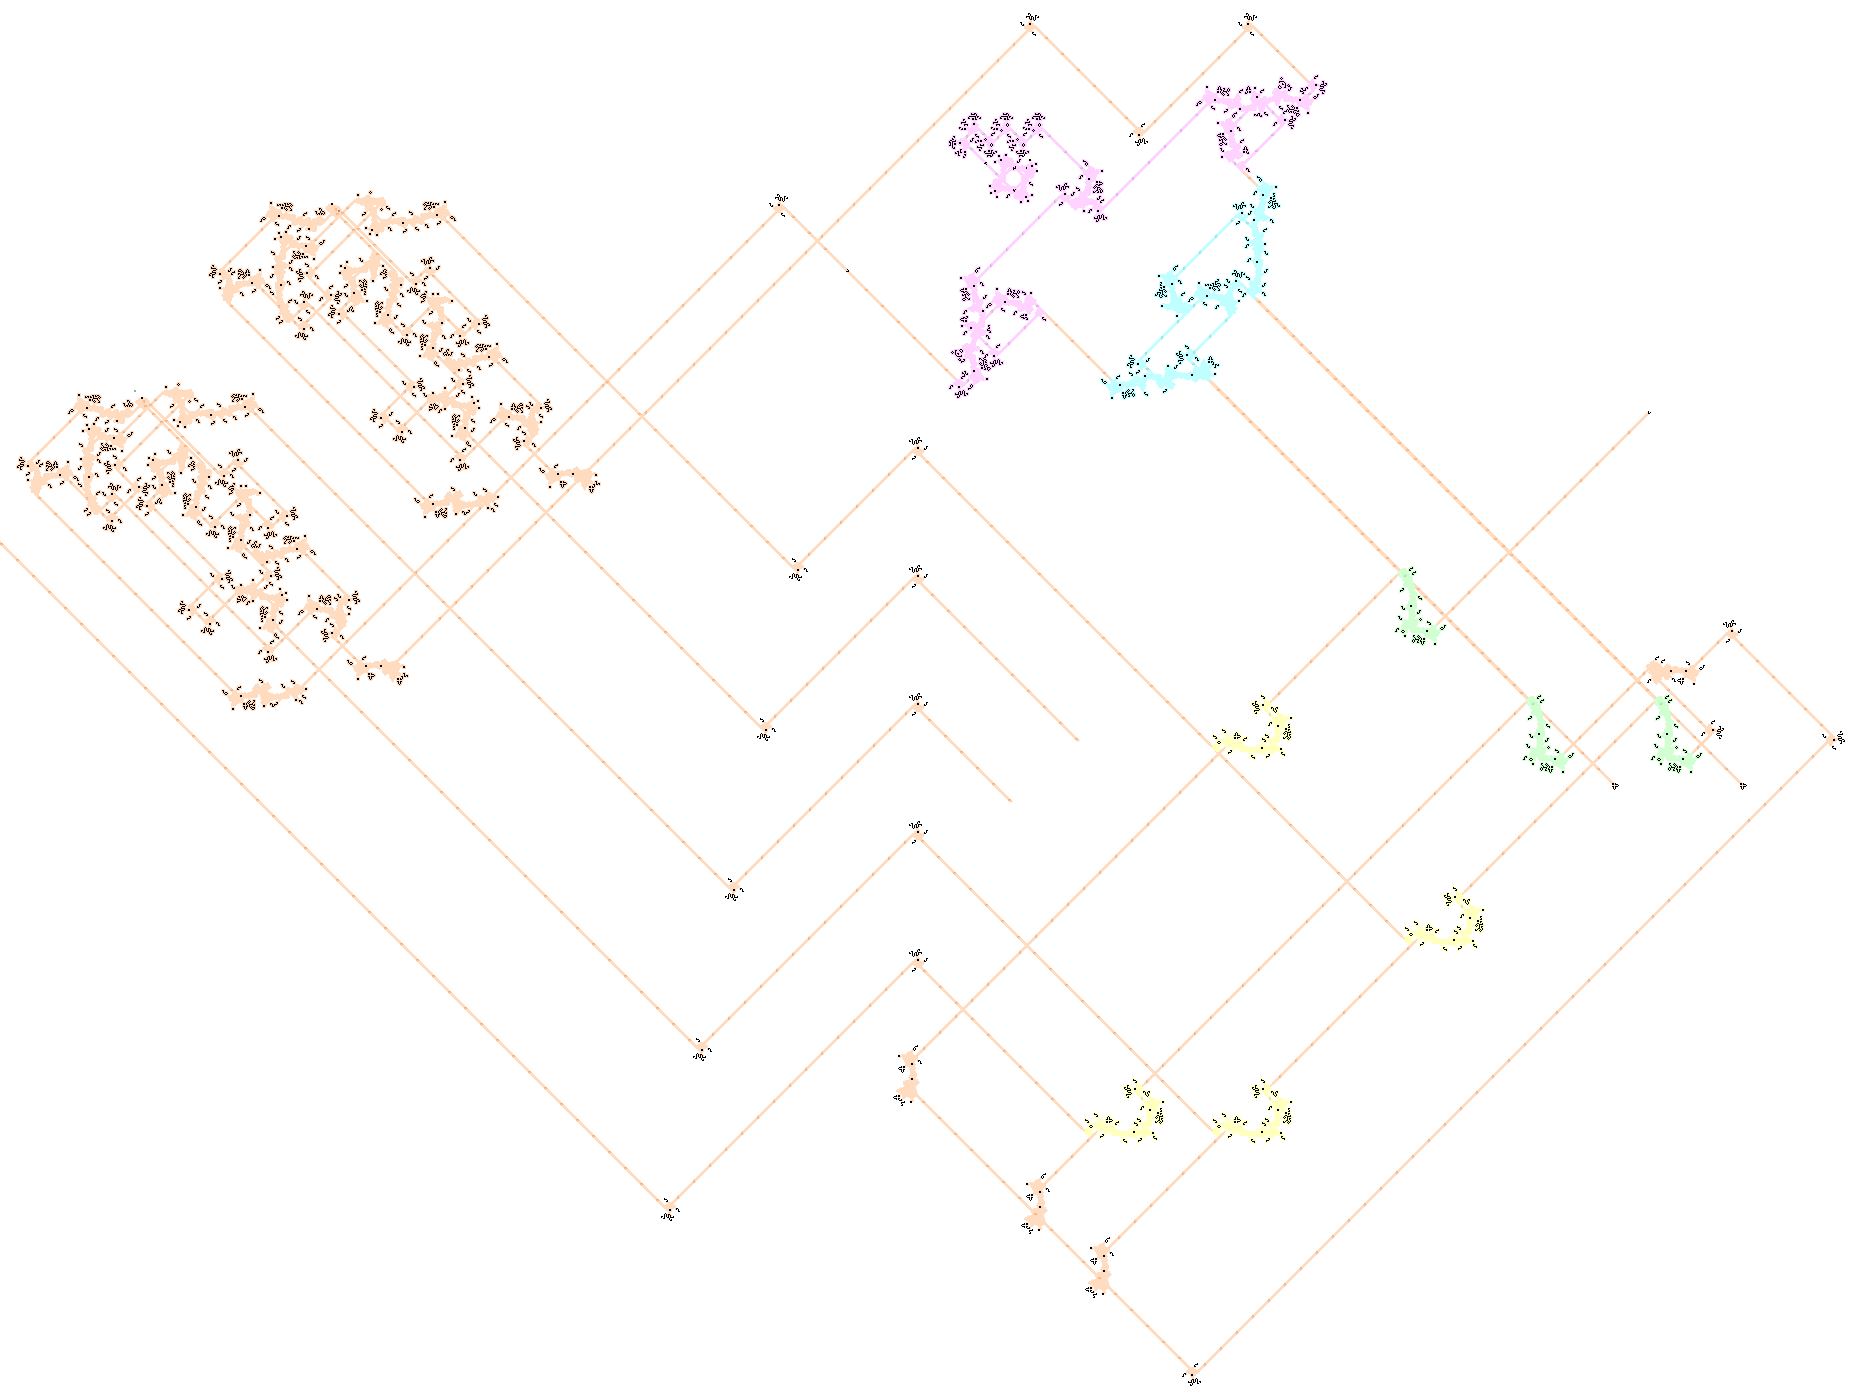
\includegraphics[width=12cm]{../universal_computation/add_computer.png}};
		
		% Z OUT
		\newcommand\zoutx{4.32}
		\newcommand\zouty{7.22}
		\draw[gray] (\zoutx,\zouty) node[rotate=45] {\tiny \texttt{Z output}};
		\draw[color=gray,-stealth] (\zoutx-0.3,\zouty-0.45) -- (\zoutx+0.5,\zouty+0.35);
		
		% NZ OUT
		\newcommand\nzoutx{5.81}
		\newcommand\nzouty{8.24}
		\draw[gray] (\nzoutx,\nzouty) node[rotate=45] {\tiny \texttt{NZ output}};
		\draw[color=gray,-stealth] (\nzoutx-0.32,\nzouty-0.45) -- (\nzoutx+0.48,\nzouty+0.35);
		
		% Z IN
		\newcommand\nzinx{8.56}
		\newcommand\nziny{6.12}
		\draw[gray] (\nzinx,\nziny) node[rotate=-45] {\tiny \texttt{Z input}};
		\draw[color=gray,-stealth] (\nzinx-0.43,\nziny+0.29) -- (\nzinx+0.37,\nziny-0.51);
		
		% NZ IN
		\newcommand\zinx{8.97}
		\newcommand\ziny{6.53}
		\draw[gray] (\zinx,\ziny) node[rotate=-45] {\tiny \texttt{NZ input}};
		\draw[color=gray,-stealth] (\zinx-0.43,\ziny+0.29) -- (\zinx+0.37,\ziny-0.51);
		
		% TDEC U0
		\newcommand\tdecrzx{5.46}
		\newcommand\tdecrzy{5.94}
		\draw[gray] (\tdecrzx,\tdecrzy) node[rotate=45] {\tiny \texttt{TDEC U0}};
		\draw[color=gray,stealth-] (\tdecrzx-0.3,\tdecrzy-0.45) -- (\tdecrzx+0.37,\tdecrzy+0.22);
		
		% INC U0
		\newcommand\inczx{5.35}
		\newcommand\inczy{5.01}
		\draw[gray] (\inczx,\inczy) node[rotate=45] {\tiny \texttt{INC U0}};
		\draw[color=gray,stealth-] (\inczx-0.3,\inczy-0.45) -- (\inczx+0.37,\inczy+0.22);
		
		% TDEC U1
		\newcommand\tdecrox{5.25}
		\newcommand\tdecroy{4.07}
		\draw[gray] (\tdecrox,\tdecroy) node[rotate=45] {\tiny \texttt{TDEC U1}};
		\draw[color=gray,stealth-] (\tdecrox-0.3,\tdecroy-0.45) -- (\tdecrox+0.37,\tdecroy+0.22);
		
		% INC U1
		\newcommand\incox{5.15}
		\newcommand\incoy{3.13}
		\draw[gray] (\incox,\incoy) node[rotate=45] {\tiny \texttt{INC U1}};
		\draw[color=gray,stealth-] (\incox-0.3,\incoy-0.45) -- (\incox+0.37,\incoy+0.22);
		
		% HALT_OUT
		\newcommand\haltx{5.05}
		\newcommand\halty{2.2}
		\draw[gray] (\haltx,\halty) node[rotate=45] {\tiny \texttt{HALT\_OUT}};
		\draw[color=gray,stealth-] (\haltx-0.35,\halty-0.5) -- (\haltx+0.42,\halty+0.27);
		
		% INITIAL; Z
		\newcommand\initzx{8.53}
		\newcommand\initzy{5.07}
		\draw[gray] (\initzx,\initzy) node[rotate=45] {\tiny \texttt{INITIAL;Z}};
		\draw[color=gray,stealth-] (\initzx-0.3,\initzy-0.45) -- (\initzx+0.42,\initzy+0.27);
		
		% ID1; Z
		\newcommand\idox{9.3}
		\newcommand\idoy{4.18}
		\draw[gray] (\idox,\idoy) node[rotate=45] {\tiny \texttt{ID1;Z}};
		\draw[color=gray,stealth-] (\idox-0.25,\idoy-0.4) -- (\idox+0.32,\idoy+0.17);
		
		% ID1; NZ
		\newcommand\idonx{9.71}
		\newcommand\idony{3.77}
		\draw[gray] (\idonx,\idony) node[rotate=45] {\tiny \texttt{ID1;NZ}};
		\draw[color=gray,stealth-] (\idonx-0.25,\idony-0.4) -- (\idonx+0.32,\idony+0.17);
		
		% CIRCLE THE INTIAL GLIDERS
		\draw[white,line width=1.5pt,opacity=0.6](5.49,7.29) circle (0.1);
		\draw[redback2,line width=0.6pt](5.49,7.29) circle (0.1);
		\draw[white,line width=1.5pt,opacity=0.6](10.673,6.36549865229) circle (0.1);
		\draw[redback2,line width=0.6pt](10.673,6.36549865229) circle (0.1);

		% COMPONENT STACK
		\draw[gridgray,dashed] (0.05,5.7) -- (0.05,6.2) -- (1.8,7.95) -- (2.8,7.95) -- (3.95,6.8) -- (3.95,5.7) -- (2.55,4.3) -- (1.45,4.3) -- cycle;
		\draw[gray] (3.4,4.8) node[rotate=45] {\scriptsize \texttt{Component Stack}};
		
		% COMPUTER
		\draw[gridgray,dashed] (5.7,1.9) -- (5.7,2.2) -- (8.1,4.6);
		\draw[gridgray,dashed] (9,5.5) -- (9.1,5.6) -- (10.8,5.6) -- (11.95,4.45) -- (11.95,4.1) -- (7.9,0.05) -- (7.55,0.05) -- (5.7,1.9);
		\draw[gray] (10.15,1.95) node[rotate=45] {\scriptsize \texttt{Computer}};
		
		% BORDER
		\draw[gridgray] (0,0) rectangle (12,9.05);
		
		% ZOOM BOX U0
			\path[draw,gridgray,line width=0.45pt] (2.102,7.8016) -- (2,10);
			\path[draw,gridgray,line width=0.45pt] (2.2965,7.8016) -- (3.552,10);
			
			\node[inner sep=0pt,anchor=north west] (zoom1) at (2,10) {
\includegraphics[width=1.552cm]{../universal_computation/add_computer_zoom1.png}};
			
			\path[fill,white,opacity=0.4,line width=0pt] (2.102,7.8016) -- (2.2965,7.8016) -- (2.2965,7.6075) -- (3.552,8.448) -- (2,8.448) -- (2.102,7.6075) -- cycle;
			
			\path[draw,gridgray,line width=0.45pt] (2.102,7.6075) -- (2,8.448);
			\path[draw,gridgray,line width=0.45pt] (2.2965,7.6075) -- (3.552,8.448);
			
			%\node[inner sep=0pt] (zoom1_3x) at (3.35,7.95) {
\includegraphics[width=0.21cm]{../mag.png} \footnotesize 8x};
			
			\filldraw[draw=gridgray,fill=white,line width=0.3pt,fill opacity=0.64] (2.102,7.8016) rectangle (2.2965,7.6075);
			\draw[gridgray,line width=0.6pt] (2,10) rectangle (3.552,8.448);
			
			\draw[gray] (2,10) node[anchor=north west] {\footnotesize \texttt{U0 = 7}};
			\draw[dred,opacity=0.5] (2.65,8.85) node[anchor=south west] {\footnotesize \texttt{0}};
			\draw[gray] (2.3,9.2) node[anchor=south west] {\footnotesize \texttt{7}};
		% END ZOOM BOX U0
		
		% ZOOM BOX U1
			\path[draw,gridgray,line width=0.45pt] (0.8539,6.6078) -- (0.1,9.5);
			\path[draw,gridgray,line width=0.45pt] (1.048,6.6078) -- (1.652,9.5);
			
			\node[inner sep=0pt,anchor=north west] (zoom1) at (0.1,9.5) {
\includegraphics[width=1.552cm]{../universal_computation/add_computer_zoom2.png}};
			
			\path[fill,white,opacity=0.4,line width=0pt] (0.8539,6.6078) -- (1.048,6.6078) -- (1.048,6.4137) -- (1.652,7.948) -- (0.1,7.948) -- (0.8539,6.4137) -- cycle;
			
			\path[draw,gridgray,line width=0.45pt] (0.8539,6.4137) -- (0.1,7.948);
			\path[draw,gridgray,line width=0.45pt] (1.048,6.4137) -- (1.652,7.948);
			
			%\node[inner sep=0pt] (zoom1_3x) at (0.92,7.58) {
\includegraphics[width=0.21cm]{../mag.png} \footnotesize 8x};
			
			\filldraw[draw=gridgray,fill=white,line width=0.3pt,fill opacity=0.64] (0.8539,6.6078) rectangle (1.048,6.4137);
			\draw[gridgray,line width=0.6pt] (0.1,9.5) rectangle (1.652,7.948);
			
			\draw[gray] (0.1,9.5) node[anchor=north west] {\footnotesize \texttt{U1 = 5}};
			\draw[gray] (0.6,8.3) node[anchor=south west] {\footnotesize \texttt{5}};
			\draw[gren,opacity=0.5] (0.2,8.7) node[anchor=south west] {\footnotesize \texttt{12}};
		% END ZOOM BOX U1
	\end{tikzpicture}
\end{document}